\chapter{Experiment setup}
\label{chapter:experiment_setup}

In this chapter we describe the data used for experiments, training setup
and experiments that were run to answer the questions asked in this thesis.

\section{\todo{Questions and constraints}}
\label{section:questions_and_constraints}

Constraints:
\begin{displayquote}
	Translation quality for multi-lingual system is insignificantly worse than for
	mono-lingual one-to-one tranlsation system.

	Maximum possible target languages are combined in one model.
\end{displayquote}

Questions:
\begin{displayquote}
	How \emph{in average} adding one more randomly selected target language
	to the multitarget model affects its En\to{}De performance?

	How is it different if we add a linguistically similar, not randomly selected language?

	How is adding one more language from the same language family or group 
	\emph{in average} affects tranlsation performance for selected language
	pair (e.g. En\to{}De)?
\end{displayquote}



\section{Experiments}
\label{section:experiments}
\subsection{Starting point}
\label{subsection:starting_point}

In \cite{johnson-etal-2017-googles} autors proposed a way to build a multi-lingual
machine tranlsation model without any changes to the \emph{Transformer} architecture.
In fact, the only change should be performed on the input data. To make the \emph{Transformer}
model process multi-lingual data the language tag is added to the source sentence.
For example, the following En\to{}Cz sentence pair:

\begin{displayquote}
Hello world! \to{} Ahoj světe!
\end{displayquote}
is modified to:

\begin{displayquote}
\tagto{cs} Hello world! \to{} Ahoj světe!
\end{displayquote}

With given method it is possible to produce translations in multiple languages using the
same model just by altering the prepended target language tag.
It was also demonstrated that this method slightly improves translation quality for 
low resource languages when compared to monolingual translation model.

In this and the following
(\perscite{arivazhagan-2019-mmnmt-in-the-wild}, \perscite{aharoni-etal-2019-massively})
papers from Google many different cases are tried and described.
However, in each setting there is usually only one model of each kind considered.
For example, when in \parcite{aharoni-etal-2019-massively} authors compare 5-to-5,
25-to-25, 50-to-50, etc. models, there is only one 5-to-5 model, one 25-to-25, etc.

Target language tags do not affect \acrshort{bleu}:
\perscite{Siddhant2019}

mNMT models en-to-4 and 4-to-en trained;
 1) \tagto{xx} added to the source;
 2) target language encoded separately.
\acrshort{bleu} scores are comparable using both approaches.


\subsection{Proposed experiments}
\label{subsection:proposed_experiments}

% Given the questions and constraints given in \ref{section:questions_and_constraints},
% the variable object in experiments is the data itself. Due to that, the setup similar
% to \cite{johnson-etal-2017-googles} was chosen. 

\subsubsection*{Bilingual baseline}

It is important to have a reference point to be able to reason how
does a change to the system affects its performance.

As a naïve and simple solution, so called \gls{baseline} system,
should be used a bilingual system with the same settings
as the systems in further experiments.

Having a performance measurement for a bilingual system in some
translation direction allows us to say about improvement or deterioration of results after
implementing a change.



\subsubsection*{n-lingual baselines (random)}

Multilingual models with random set of languages.
The purpouse is twofold: 
to show \acrshort{bleu} score decrease with increasing number of target languages and
to serve as a baseline for multitarget models with target languages grouped by
in non-random way, e.g. by language group or linguistic similarity.


\subsubsection*{Group by language group}

If all target languages are from one language group we expect to observe
better translation quality comparing to multilingual baseline results 
with randomly selected target languages.
This is expected due to shared parts of vocabulary (todo: expand with examples)
and linguistic properties (again, expand with examples).
Germanic group: da, de, is, no, nl, sv.
Slavic with cyrillic script: bg, mk, ru, uk.
Slavic: bg, cs, hr, mk, pl, ru, sk, sl, sr, uk


% \subsubsection*{Group by linguistic similarity}
% 
% From \perscite{siddhant-2020-x-ling-effect} follows that languages' script
% and similarly the amount of shared vocabulary is not so important
% for XX\to{}En translation direction.
% Example with Serbian and Croatian, with the same vocabulary but
% in different scripts.





\section{Dataset(s)}
\label{section:datasets}


\subsection{\edit{English to 36 languages}}
\label{subsection:en-to-36}

To observe effects of linguistic similarity of target languages
it is important to examine enough possible variations of those.
The OPUS dataset (\cite{TIEDEMANN12.463}) is an open and free collection of texts
that covers more than 90 languages with data from several
domains.\footnote{Available at \url{http://opus.nlpl.eu/}} 

For our experiments the source language is English only.

Sampling and splitting of the data is the one used for
ELITR project.%
\footnote{\url{https://elitr.eu/wp-content/uploads/2019/07/D11.FINAL\_.pdf}}
For each of language pairs and each sub-dataset
the data was splitted to training, validation and testing sets.
For each of the two latter sets 2000 random sentences were selected
and the rest of the data remained for the training set.
In cases where the sub-dataset contained less than 16000 sentence pairs
no data went to the validation set.
Later for each language pair there were 1000000 sentence pairs
sampled from all training sub-sets.
Firstly, if available, the sentences were taken from Europarl,
then EUbooks, OpenSubtitles, and then all remaining sub-datasets.
The same procedure was used to sample x000 of validation set sentences
per each language pair.
The test sets were left separate, so that the result on each domain would be observable.

Later an overlap in the source side of different language pairs was found.
Although this would not directly lead to unfair increase of the test score,
such sentence pairs were removed from the training sets.
This filtering decreased the amound of sentence pairs
to 0.85-0.95 millions per language pair.

\begin{figure}[h]
	\centering
	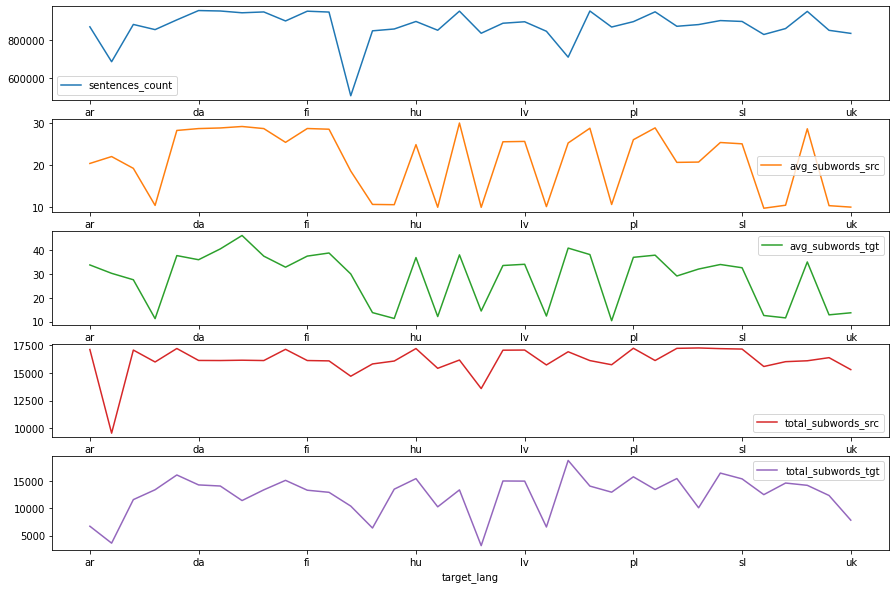
\includegraphics[width=0.9\columnwidth]{../img/train_set_statistics.png}
	\mycaption{Training data language statistics}{
		Languages are on the \emph{X} axis sorted as in appendix.
		From top to bottom:
		total number of sentence pairs in training set per language,
		average amount of subwords per sentence on the source side,
		the same on the target side,
		total amount of unique subwords for this target language on the source side,
		the same on the target side.
	}
	\label{fig:language_statistics}
\end{figure}


\begin{table}[h!]
	\centering
	\begin{tabular}{c|p{0.5\columnwidth}|p{0.4\columnwidth}}
	\toprule
	     group & subdataset names  & description \\
	\midrule
	 1 &  Europarl/vx, DGT, MultiUN, EUbookshop, JRC-Acquis,
	      ECB, EMEA
	   &  Proceedings and documents from Europarl, UN, etc. \\
	 2 &  NewsCommentary, GlobalVoices, WMT-News 
	   &  News articles and commentaries \\
	 3 &  OpenSubtitles, Tatoeba
	   &  Short sentences, human speech, general domain \\
	 4 &  OpenOffice, PHP, KDE4, Gnome
	   &  Software documentation or interface elements \\
	 5 &  Bible, Tanzil, Books 
	   &  Other: completely different domain, dated vocabulary
	      automaticaly aligned sentences, etc. \\
	\bottomrule
	\end{tabular}

	\mycaption{Groups of subdatasets in OPUS}{}
	\label{tab:subdatasets_groups}
\end{table}


\subsection{\todo{UN parallel corpus: English to 5 languages}}
\label{subsection:en-to-5}

\todo{as I show en-to-5 results in RANDOM section, this DS should be here}
\cite{eisele-chen-2010-multiun}


\section{Method}
\label{section:method}

In this section we describe how the models are trained, which metrics
are collected and how are they analyzed.

\subsection{\edit{Training}}

For example, let us take En\to{}$\{$Fr, De$\}$ setup, which means that
the model to be trained should take a source sentence in English and
produce translation either in French or in German.
The language of model's translation depends on the target tag at the beginning
of the input sentence, i.e. \tagto{fr} tag in source sentence leads to French
translation.

To train such a model, only related sentence pairs are subsampled
from the whole training set.
In this case, from the whole training set we select only those sentence
pairs which source side starts with tags \tagto{fr} or \tagto{de}.
Such subsampled dataset is then used to train the model.

During the training procedure, once per specified number of updates
occurs the checkpointing of the model.
The model weights are saved to the disc and number of metrics are logged.

\begin{samepage}
\begin{itemize}
	\item [Those metrics are:]
	\item training loss value (mean value for all updates since
	last checkpoint)
	\item current learning rate value
	\item training speed (processed words per second)
	\item training time since last checkpoint
	\item current number of updates
\end{itemize}
\end{samepage}
\begin{samepage}
Hardware usage should also be recorded if possible:
\begin{itemize}
	\item GPU usage
	\item CPU usage
	\item memory usage
	\item disc I/O
	\item network I/O
\end{itemize}
\end{samepage}

The hardware metrics are not important for model's evalueation
but may help early spot mistakes like underuse of GPU or CPU, lack of RAM, etc.

\subsection{\edit{Validation}}
\label{subsection:validation}

The validation set is used to track model's performance
on an unseen set of data and to perform early stopping.
Once per specified number of steps the validation occurs:
validation metrics are recorded, for any metric which value was
improved current model weights are saved as best model by this metric.
If early stopping condition occured then the training process is stopped.

For any model the validation set is constructed of the big validation set
by selection only relevant sentence pairs in the same way, as the training set.

For the example setup from above, En\to{}$\{$De,Fr$\}$, the validation set
consists of equal amount of En\to{}De and En\to{}Fr sentence pairs.
E.g. if in the complete validation set there are 1000 sentence pairs for
each of possible target languages, then for En\to{}$\{$De,Fr$\}$
model the validation set will contain 2000 sentence pairs, and for
En\to{}$\{$De,Es,Fr$\}$ it will contain 3000 sentence pairs.

For the validation set we collect not only the loss function value
but also the metric of interest, which is \acrshort{bleu} score.
However, the \acrshort{bleu} of the whole model's validation set
is not something we are interested in.
For the discussed example we collect bleu:fr and bleu:de scores
which represent \acrshort{bleu} scores for French and German
parts of validation set.
E.g., to compute bleu:fr we select only En\to{}Fr sentence pairs from the
validation set.

Also, an aggregated value of the bleu:xx scores is also recorded
and may be used for early stopping: ending the training process
when the metric is not improved during last N validation steps.

\begin{samepage}
All together, the following validation metrics are recorded after the
validation step:
\begin{itemize}
	\item loss function value
	\item bleu:xx which is \acrshort{bleu} score for each of
	model's target languages
	\item aggregated value of all bleu:xx values
	\item translation time of the model's validation set
\end{itemize}
\end{samepage}

\subsection{\todo{Finishing the training}}
\label{section:finishing-the-training}

When should we stop the training?
It is not possible to say precisely when did the model
acquire its best performance because of stochastic nature of
the training algorightm (\acrshort{sgd}).
Because of that we need to use some method how to decide when
training process should be stopped.


\subsubsection*{Number of \glspl{epoch}}

\todo{First occurance of a term to be italic}
The easiest approach is to specify number of \glspl{epoch}
after which the training is stopped.
This could be a good solution for the case when all models
that will be compared are trained on the same amount of data from
the same domain.
But in our case, adding one more target language adds a constant
amount of sentence pairs to the training set.
Roughly, if the number of \glspl{epoch} is specified as a stop
condition, a bilingual \dir{En}{De} model will see the German
training data $x$ times, when multilingual \dir{En}{De, Fr, Es}
will only see the German training data $x / 3$ times.

%What value should be used to compare model's performace in time?
%The first and the most obvious approach 
\subsubsection*{Early stopping}

\Gls{early-stopping} is a regularization technique used to avoid
possible \gls{overfitting} of a model on the training data.
In general, it works in the following way: after every validation step
it checks if the metric value improved during last $N$ validations.
The metric to be controlled and number of validation steps $N$ are
the parameters of this method
(Figure \ref{fig:early_stopping}).

Another situation is even more probable: model's validation performance
is either stalled or slightly improved
(Figure \ref{fig:early_stopping_no_improvement}).
In this case \gls{early-stopping} helps to avoid unnessecery spendings
on computational resources.

\begin{samepage}
\begin{figure}[h]
	\centering
	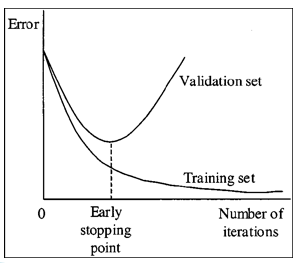
\includegraphics[width=0.6\columnwidth]{../img/early_stopping.png}
	\mycaption{\Gls{early-stopping} to prevent overfitting}{
		At the 'early stopping' point the model's performance
		on unseen validation set of data does not improve
		anymore. Further training leads to poorer performance
		on unseen data. Stopping the training at this point
		results in better model's performance on unseen data.
	}
	\label{fig:early_stopping}
\end{figure}

\begin{figure}[h]
	\centering
	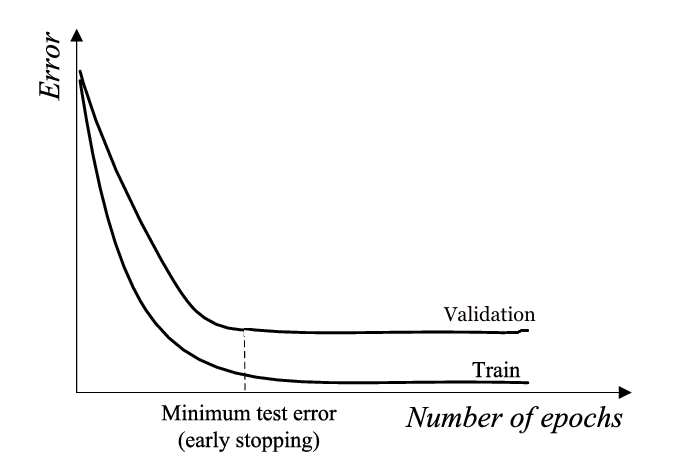
\includegraphics[width=0.6\columnwidth]{../img/early_stopping_no_improvement.png}
	\mycaption{\Gls{early-stopping} as the model is not improving}{
		Even though the metric value on the training set is
		still slowly improving, the its value on the unseen
		validation set is stalled. Further spending of 
		computational resources is unjustified.
	}
	\label{fig:early_stopping_no_improvement}
\end{figure}
\end{samepage}

In our case we could use \gls{early-stopping} to ensure more equal conditions
for models with different sizes of training data. Suitable number $N$
could be found experimentaly, but which metric should be used?

\todo{cross-entropy, perplexity; they may not represent the model's
performance, what about BLEU}

Given that the task is to train a model that is as good as possible in
\textbf{every} of its target directions, the \acrshort{bleu} score of
the whole translated validation set for this set of languages does not
say anything about the model's performance in each specified
translation direction.

\subsubsection*{Aggregated value of BLEU scores}

Therefore, we should use separate BLEU scores which represent
model's performance in each of translation directions.
The most intuitive and naive way is to compare BLEU scores
for each target language.
But if we will try to set up an early stopping on each of the values,
the following may happen: BLEU for on of the directions will stay the
same for long enough to trigger early stopping, but for another direction
the BLEU score is still growing.

For example, suppose the model is being trained for \dirmany{En}{De, Fr}
and validation happens after each 1000 update steps.
At the step 20000 for some selected German validation set
the model's \dir{En}{De} performance measured by BLEU score
equals 20, for the \dir{En}{Fr} direction its BLEU score is 15.
After 10 more validations, model's performance for \dir{En}{De}
is still equal to 20 BLEU and did not grow, but for \dir{En}{Fr} 
it has already reached 25 and is still increasing.
Early stopping will be triggered, and even though the performance
in \dir{En}{De} direction might have reached its possible maximum
(assuming that the early stopping period of 10 checks was selected
efficiently) its \dir{En}{Fr} performance might still improve.

\todo{Geometric mean: good for multiple metrics with different scale}


\subsection{\edit{Testing}}
\label{subsection:testing}

After the training is finished, the received models should be evaluated on unseen
test data.
For experiments with \gls{en-to-5} dataset (Section \ref{subsection:en-to-5})
the test sets are created in the same way as validation sets.
For \gls{en-to-36} dataset (Section \ref{subsection:en-to-36})
the test set is divided on subsets by the source dataset.
It means, that each of source datasets (like OpenSubtitles/v11, 
Europarl/v7, etc.) there exists a separate test set.
So after translating the test set for each of target directions of the model
the following record is created:
\begin{itemize}
	\item model name
	\item source language
	\item target languages
	\item tested target language
	\item \acrshort{bleu} score for this part of translation
	\item metric, based on which the best model was saved
	\item dataset name (for \gls{en-to-36})
\end{itemize}

Let us return to the example setup is En\to{}$\{$De, Fr$\}$ and
suppose the reported validation metrics are the mean loss function value on
test set and 'translation' (geometric mean of all reported BLEU scores,
see Section \ref{subsection:validation}).
After the training is finished, there will be two models: best by
loss value and best by 'translation'.
For each of those two records are created: for En\to{}Fr translation
and for En\to{}Es. In total, 4 results are recorded.

If the model was trained and tested on \gls{en-to-36} dataset,
than 4 times \textit{n} records are created, where \textit{n}
is number of OPUS subdatasets from which the data was sampled.


\subsection{\todo{Analysis}}

After required set of models is trained and their test
metrics are collected, data should be analysed.





\section{Training tools}

In the following section we describe the tools that are uset to implement
what was shown in Section \ref{section:method}.

\subsection{Tool kits}

There exists a number of different tools that can be used for training a NMT model.
General purpouse deep learning programming libraries like
Tensorflow\footnote{\url{https://tensorflow.org/}} and
PyTorch\footnote{\url{https://pytorch.org/}} are most popular for deep learning related
research. With their help it is possible to construct any of today's state-of-the-art
NMT models; pre-built and pre-trained models are initially present in such frameworks,
but it is also possible to describe a model from scratch.

Another option is presented by specialized NMT tool kits.
They usually contain efficient and tested implementations of NMT models as well as some of
usefull preprocessing tools.
For the experiments described in \ref{section:experiments} there is a need to train significant
amount of models with the same architecture and settings but different datasets.
Due to that fact, in this work the use of specialized NMT tool kit is more suitable.
Let us consider the foolowing list of broadly used tool kits as for year 2020,
presented in \cite{koehn_2020}:

\begin{itemize}
  \item OpenNMT (based on Torch/pyTorch)\footnote{\url{https://opennmt.net}}
  \item Sockeye (based on MXNet)\footnote{\url{https://github.com/awslabs/sockeye}}
  \item Fairseq (based on pyTorch)\footnote{\url{https://github.com/pytorch/fairseq}}
  \item Marian (stand-alone implementation in C++)\footnote{\url{marian-nmt.github.io}}
  \item Google's Transformer (based on Tensorflow)\footnote{\url{
    https://github.com/tensorflow/models/tree/master/official/transformer}}
  \item Tensor2Tensor (based on Tensorflow) \footnote{\url{
    https://github.com/tensorflow/tensor2tensor}}
\end{itemize}

We chose \textit{MARIAN-NMT} tool kit\footnote{\cite{mariannmt}} as a fast solution
with stable and efficient \textit{Transformer} \cite{vaswani-2017-transformer} implementation,
minimum of third-party dependencies, and ability to train models on multiple GPU units in parallel.


\subsection{Computational cluster}

In the experiments proposed above the expected number of models to be trained is quite big.
First of all, there should be 36 models for \textit{mono-target baseline} for En\to{}36 dataset.
For \textit{multi-target random} experiment the number is much bigger.
For example, let us consider a case with En\to{}3 models - each model translates from English to 
3 target languages. Specifying that each of 36 target languages from En\to{}36 dataset
should appear at least in 3 En\to{}3 models, series of random generation of En\to{}3 setups gave
the smallest amount of such setups equal to 44. For En\to{}5 case with 5 target languages in each
model and with the same restriction of minimum occurance the same procedure gave the
minimum amount of needed models equal to 34.

To be able to train large number of models in a reasonable amount of time we needed to use
computational cluster with GPU cards.
The computational clusters available at the institution are operating under
SGE\footnote{\url{https://arc.liv.ac.uk/trac/SGE}} scheduling software and are equipped with
GPU cards with minimum CUDA \textit{compute capability} 6.1.

Considering data storage quota limitation and high utilization of computational resources by
the cluster's users, the following training pipeline was designed:

\begin{outline}
    \1 Prepare task list
    \1 Iterate over the list working with at most N tasks in parallel
    \1 For each task
        \2 Subsample the dataset taking only those sentence pairs with target languages
	   specified in the task
	\2 Run the training procedure for limited amount of time (e.g. for one hour only)
	   starting with previous checkpoint if it already exists
	\2 Regularly compute metrics on the developement set and report them
	\2 On the event of evaluation on the developenemt set save the best model for each metric
	\2 After time is out the training is stopped and subsampled datasets are removed
    \1 If for next selected task the model is already trained then select next task from the list
    \1 If for next selected task the model is currently being trained then decrease
       the number N of tasks processed in parallel
\end{outline}


\subsection{Inspecting the training process}

As the number of models trained and being trained is growing, monitoring of the training
process becomes more and more complicated. If the experiments are also being run on different
computational clusters it becomes very possible that a parameter mistakenly set up to different
value or a corrupted dataset, or even hardware version may lead to an unexpected difference in results.

To address these and other issues that may occur during the training process we use
Weights$\&$Biases\footnote{\cite{wandb}} experiment tracking tool.
Its main features that are useful in this prospective are following:
\begin{outline}
	\1 Metric visualization
		\2 Training and validation loss curves
		(Figure \ref{fig:single-lang-group-vs-random-dashboard} left subplot)
		\2 Scatter plots (Figures \ref{fig:inspect-convergence}
		and \ref{fig:single-lang-group-vs-random-dashboard} middle subplot)
	\1 Artifact storage
		\2 Model checkpoints storage
			\3 stores 'heavy' model files which cannot be stored
			in \emph{git}
			\3 along with \emph{git} it makes possible to move training
			to the different computational cluster system
		\2 Sample translations of validation set
			\3 helps to observe improvements of translation quality
			in time
			\3 lets verify that model is actually produces meaningfull
			translation
	\1 Customizable reports
	\1 Hardware utilization
\end{outline}

\begin{figure}[h]
	\centering
	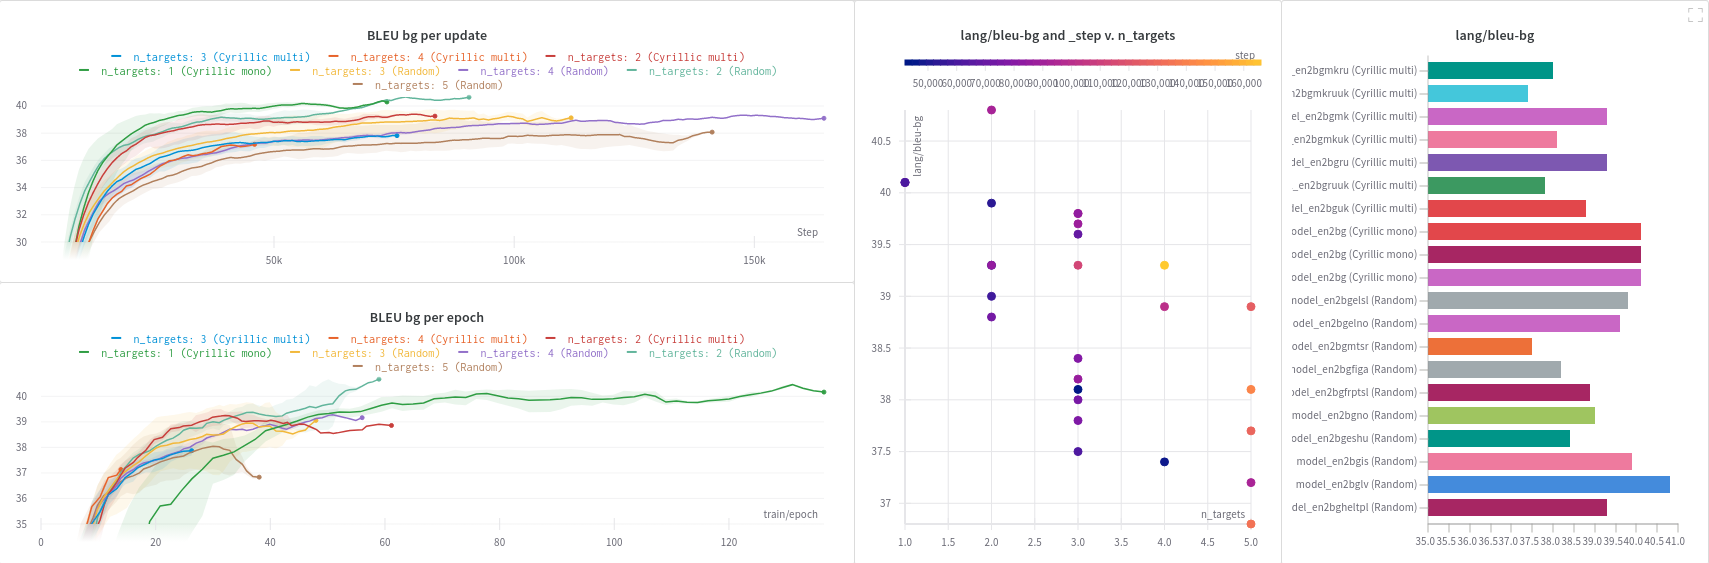
\includegraphics[width=1.0\columnwidth]{../img/slavic_cyrillic_bg.png}
	\mycaption{%
		Single language results visualization: models other
		target languages are randomly selected
		vs. those selected from similar group of languages%
	}{
		\todo{split it in print-friendly way}
		Here is a part of interactive report for 'slavic languages with cyrillic script vs. random'
		experiment. In this specific case models' performace on Bulgarian part of
		validation set is compared.

		\emph{Left}: \acrshort{bleu} score for En\to{}Bg translation direction is monitored with
		training step on \emph{X} axis (top) and training epoch  (bottom).
		Each curve represents mean value (line) and its min/max value
		(range) at the point of time of multiple models' results.
		Models are grouped by number of target languages and experiment subgroup
		(En\to{}Bg, En\to{}Slavic and En\to{}Random).

		\emph{Middle}: Number of targets (axis \emph{X}) vs.
		\acrshort{bleu} on En\to{}Bg validation set (axis \emph{Y}) vs.
		update steps (colos with scale at the top).

		\emph{Right}: Individual models' En\to{}Bg validation \acrshort{bleu} scores.
	}
	\label{fig:single-lang-group-vs-random-dashboard}
\end{figure}


\begin{figure}[h]
	\begin{minipage}{0.8\textwidth}
	\centering
	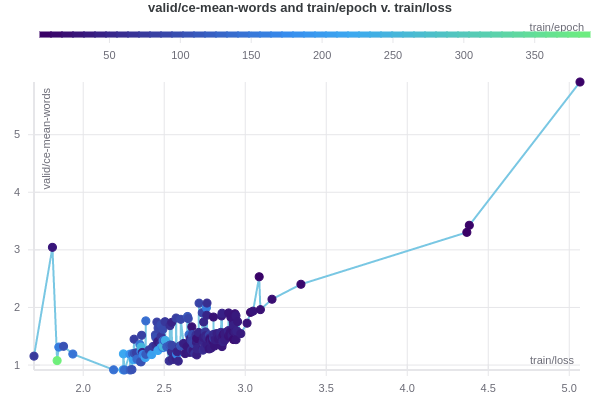
\includegraphics[width=1.0\columnwidth]{../img/inspect_overfit.png}
	\end{minipage}\hfill
	\begin{minipage}{0.8\textwidth}
	\centering
	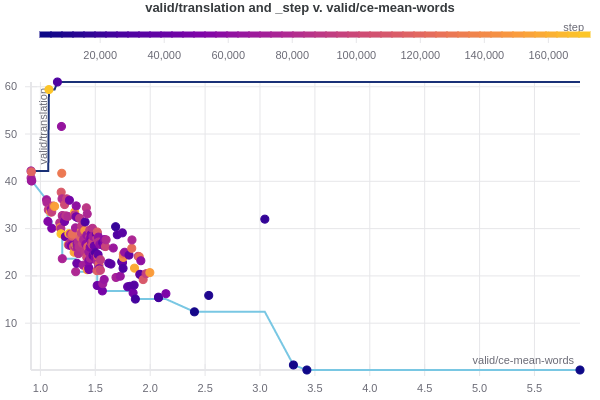
\includegraphics[width=1.0\columnwidth]{../img/inspect-bleu-vs-loss.png}
	\end{minipage}
	\mycaption{%
		Overall model convergence dashboard%
	}{
		On these two interactive graphs each point represents one model.
		Models that are currently training are visualized here together with
		completely converged models and those which training process is currently
		on hold.

		\emph{Left}: axis \emph{X} represents the training loss value,
		axis \emph{Y} represents the value for the same loss function calculated
		on the validation set. The color of each point represents current training
		epoch for the model. Normally for any model the point moves from top right
		part of this graph to the bottom left part, representing both training and
		validation loss being gradually decreased during the training procedure.
		The point that moves to the middle left part of the graph may signalize about
		either \gls{overfitting} of the model on training set, or difference in data
		distribution in training and validation set, or else some mistake in training
		settings.

		\emph{Right}: on this plot loss value on the validation set (axis \emph{X})
		is compared with geometric mean of \acrshort{bleu} scores
		for each of target languages.
		For any model during the training procedure its point usually moves from
		bottom right corner into the cluster of other points.
		Model which point 'arrives' to any other location than the cluster may need
		special attention.
	}
	\label{fig:inspect-convergence}
\end{figure}



\subsection{\todo{Model settings}}

The initial parameter selection is made with respect to \cite{training-tips}.
First of all, the hyperparameters of MT model are tuned
on couple of language pairs from one dataset.
The parameters leading to the same result in shorter time were preferred.
Then the selected parameters were used on all experimends with the dataset.


\subsubsection*{Tuning early stopping on early runs}

The initial \gls{early-stopping} setting was that after 5 consecutive
validation steps without improvement of validation \gls{loss} value
the training process stopped.
However, during the training of first couple of bilingual models the following
situation have happened quite often.
Further improving performance on validation set by
couple of tenths of BLEU points took as much time as reaching the optimal state.

On the Figure \ref{fig:no_improvement_de} can be seen that path from
the beginning of training to optimal point B (26.9 \acrshort{bleu})
took as much time as its further improvement by 0.2 BLEU
at point D (27.1 \acrshort{bleu}). However, there were certain models
with a bit bigger improvement after a much longer time, e.g.
0.8 \acrshort{bleu} points on Figure \ref{fig:no_improvement_fi}.

Possible situations of this kind were discussed in
Section \ref{section:finishing-the-training}.
After considering also some of preliminary multilingual runs
the 'patience' parameter of \gls{early-stopping} was set to 15.
After 15 consequent validation steps without metric improvement
the training process is stopped.

\begin{figure}[p]
	\centering
	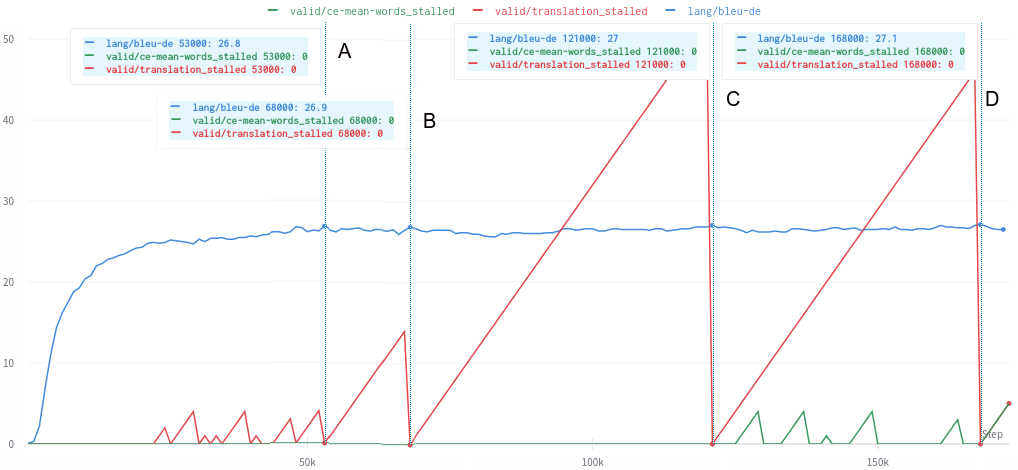
\includegraphics[width=1.0\columnwidth]{../img/no_improvement_de.png}
	\mycaption{Example change of model's performance on validation set
		   in time}{
		Preliminary \dir{En}{De} model.

		\textit{Blue}: validation metric (value on the left axis in BLEU)

		\textit{Red}: validation metric (BLEU) stalled.
		Each consecutive validation step when the metric
		is not improved this value is incremented by 1.
		When the metric is improved this value is reset to 0.

		\textit{Green}: loss function value on validation set is
		stalled. Same logic as for \textit{Red}.

		BLEU score values at the points of improvement:
		$A$ -- 26.8, $B$ -- 26.9, $C$ -- 27.0, $D$ -- 27.1.
	}
	\label{fig:no_improvement_de}

	\vspace*{\floatsep}% https://tex.stackexchange.com/q/26521/5764

	\centering
	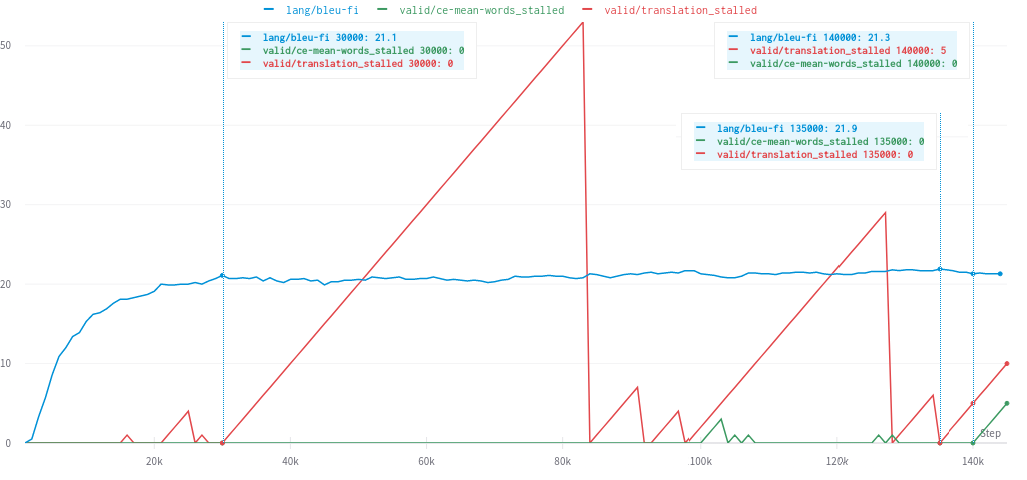
\includegraphics[width=1.0\columnwidth]{../img/no_improvement_fi.png}
	\mycaption{Small improvement during long training}{
		In this case (\dir{En}{Fi}) the difference is a bit more
		visible: 21.3 at the first point and 21.9 at the best.
		Colors and scales are the same as at
		Figure \ref{fig:no_improvement_de}.
	}
	\label{fig:no_improvement_fi}
\end{figure}
